% riprendere qualcosa dalle slide Fiormonte Ciotti (Introduzione alla codifica XML per i testi umanistici)

% Il computer si è dimostrato un potente strumento per redigere, conservare, diffondere, analizzare i testi.
% % dalla slide vitali
% The ecosystem of text
% • Editing
% • Validating
% • Printing & displaying
% • Transforming and converting
% • Annotating
% – Annotating annotations
% • Searching
% • ... 



% detta difficile: “riconoscere un fenomeno dato come il token di un dato type presuppone alcune ipotesi sul contesto espressivo e sul co-testo discorsivo” (Eco)

% La codifica elettronica dei testi ha rappresentato uno dei temi fondamentali della riflessione e della sperimentazione nel dominio dell’Informatica umanistica.

% ad oggi la soluzione considerata ottimale per una corretta rappresentazione del testo è l'adozione dei markup language descrittivi basati su XML


\begin{frame}
	\frametitle{Rappresentazione digitale dei testi}
	\framesubtitle{basso e alto livello di codifica}
	\addtocounter{nframe}{1}

	\begin{block}{Codificare un testo}
		La codifica dei caratteri evidentemente non esaurisce i problemi per una opportuna rappresentazione delle caratteristiche interne ed esterne di un testo.
    \end{block}
    
    \begin{block}{Codificare un testo}
		Di fatti la codifica del testo è una questione molto più complessa di una semplice riproduzione meccanica di un dato.
	\end{block}


\end{frame}


\begin{frame}
	\frametitle{Rappresentazione digitale dei testi}
	\framesubtitle{basso e alto livello di codifica}
	\addtocounter{nframe}{1}

	\begin{block}{Rappresentare un testo}
		
			La rappresentazione digitale di un testo è una operazione intrinsecamente assai difficile perché coinvolge una pletora di aspetti a vari livelli di astrazione, a varie dimensioni e a varie granularità sia teorici, sia metodologici, sia tecnologici e sia pratici.
		
	\end{block}

\end{frame}

\begin{frame}
	\frametitle{Rappresentazione digitale dei testi}
	\framesubtitle{basso e alto livello di codifica}
	\addtocounter{nframe}{1}

	\begin{block}{Rappresentare un testo}
		\textbf{
			Prima di poter fare qualsiasi ipotesi su come compiere una codifica di un testo e su come rappresentarlo digitalmente, bisogna stabilire, infatti, cosa si intende per testo.
		}
	\end{block}

\end{frame}


\begin{frame}
	\frametitle{Rappresentazione digitale dei testi}
	\framesubtitle{Modello dati di un testo}
	\addtocounter{nframe}{1}

	\begin{block}{Un testo non ha una struttura rigida, predefinita: }
		\begin{itemize}

			\item Non è rappresentabile solo come un insieme di record di un archivio elettronico.
			\item Non è rappresentabile solo come un insieme di tabelle di una banca dati.
			\item Non è rappresentabile solo come un albero o un insieme di sotto-alberi
			\item Non è rappresentabile solo come un grafo o come un insieme di sotto grafi

		\end{itemize}

	\end{block}

\end{frame}

\begin{frame}
	\frametitle{Molteplici modelli per diverse esigenze}
	\framesubtitle{Strutture dato e testo}
	\addtocounter{nframe}{1}

	\begin{block}{La rappresentazione di un testo}
		\begin{center}
			 %mia slide sulle possibili rappresentazioni del testo
			- lineare: sequenza di dati non strutturati
			\\- records: enumerazione delle proprietà
			\\- tabulare: insieme di dati omogenei
			\\- albero: gerarchie di dati e insiemi di dati
			\\- grafo: rete di strutture informative interconnesse tra loro
        \end{center}
        
	\end{block}
    [SLIDE DA COMPLETARE]
\end{frame}



\begin{frame}
	\frametitle{Elementi di Codifica del testo}
	\framesubtitle{Formalismi}
	\addtocounter{nframe}{1}

	\begin{block}{Formati di rappresentazione}
		\begin{center}
			Un formato è un insieme di regole e convenzioni formali per rappresentare un insieme di dati, nel nostro caso un testo.
		\end{center}

	\end{block}

	\begin{block}{Importanza dei formati}
		\begin{center}
			Seppur isomorfi la scelta di un formato condiziona molto l'efficienza delle operazioni e l'efficacia delle dichiarazioni.
		\end{center}

	\end{block}


\end{frame}

%\begin{frame}
%    \frametitle{Elementi di Codifica del testo}
%    \framesubtitle{lista di formati}
%    \addtocounter{nframe}{1}
%   
%    \begin{block}{Formati dato}
%Data structures – CSV and tabular data
%– JSON
%– RDF
%Plain text formats – Plain text
%– TeX, LaTeX, etc.
%– Markdown, CommonMark and wiki syntaxes
%Markup formats
%– HTML, HTML5
%– XML
%– HTML5+ Embedded annotations (e.g., HTML5 + RDFa)
%– Markup spinoffs for overlapping (e.g. LMNL, TexMECS, etc.) 
%
%    \end{block}

% \begin{block}{Riferimenti TEI}
%     Capitolo sul character encoding e modulo Ganji 
% \end{block}

%\end{frame}

\begin{frame}
	\frametitle{Elementi di Codifica del testo}
	\framesubtitle{Tabella Formalismi}
	\addtocounter{nframe}{1}

	\begin{block}{Formalismi}
		\begin{center}
			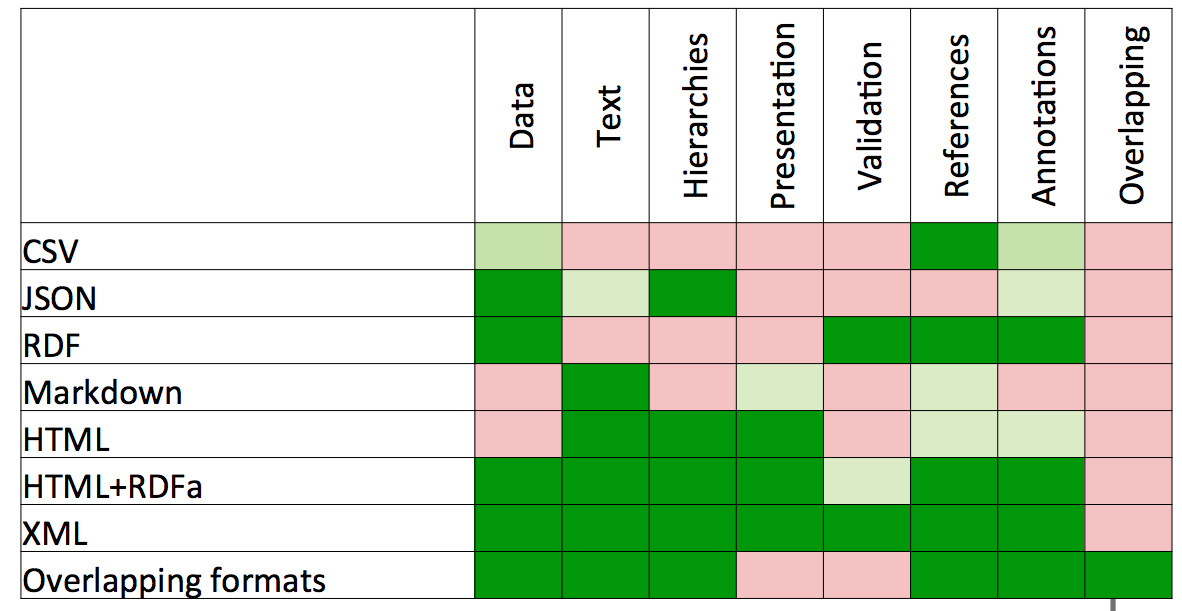
\includegraphics[width=.9\textwidth]{imgs/TabellaFormalismiCodificaTesto.png}
		\end{center}
	\end{block}
	courtesy of \textit{Fabio Vitali}

\end{frame}


\begin{frame}
	\frametitle{Elementi di Codifica del testo}
	\framesubtitle{Formalismi}
	\addtocounter{nframe}{1}

	\begin{block}{Formati come formalismi}
		\begin{center}
			Data l'importanza metodologica il formato del dato diviene un vero e proprio formalismo, si parla cioè di linguaggi di codifica in quanto questi sistemi si basano su un insieme di istruzioni rigorose di codifica.
		\end{center}

	\end{block}

\end{frame}



\begin{frame}
	\frametitle{Elementi di Codifica del testo}
	\framesubtitle{Formalismi}
	\addtocounter{nframe}{1}

	\begin{block}{Formati e formalismi di codifica}

		Quindi ogni pezzo di informazione aggiunta ad un testo grezzo attraverso l'inserimento di dati metatestuali (markup, annotazione, codifica), constituisce il risultato di una analisi e di una interpretazione che è stata condotta (da un umano o da una macchina) al fine di esplicitare e rappresentare nel modo più accurato possibile le informazioni da veicolare attraverso il formato digitale prescelto (anche in modo incrementale).


	\end{block}

\end{frame}





% % altra slide Vitali
% • Text has characters, including punctuation
% – We all (sort of) agree on this
% • Texts is ordered
% – In ``To be or not to be'', it is important that ``To be''
% comes before ``not to be''
% • Text has structure
% • Text has presentation
% • Text has grammar
% • Texts has semantics
% • Text has variants
% • Text has a lot of things that can be said about it 
